\documentclass{article}
\usepackage[utf8]{inputenc}
\usepackage[italian]{babel}
\usepackage{verbatim}
\usepackage{geometry}
\usepackage{enumitem}
\usepackage{ccicons}
\usepackage{setspace}
\usepackage{hyperref}
\usepackage{xcolor}
\usepackage{tikz}
\usepackage{graphicx}
\usepackage{siunitx}
\usepackage{amsmath}





\geometry{left = 2 cm, right = 2 cm, bottom = 2 cm, top = 2.5 cm}
\setlength{\parindent}{0em}
\hypersetup{
    colorlinks,
    linkcolor={black},
    citecolor={black},
    urlcolor={black}
}

\pagestyle{plain}
\pagenumbering{gobble}

\title{\Huge Electric Circuits Exercises}
\author{}
\date{}
\begin{document}
\maketitle
\vspace{2cm}
\begin{figure}[h]
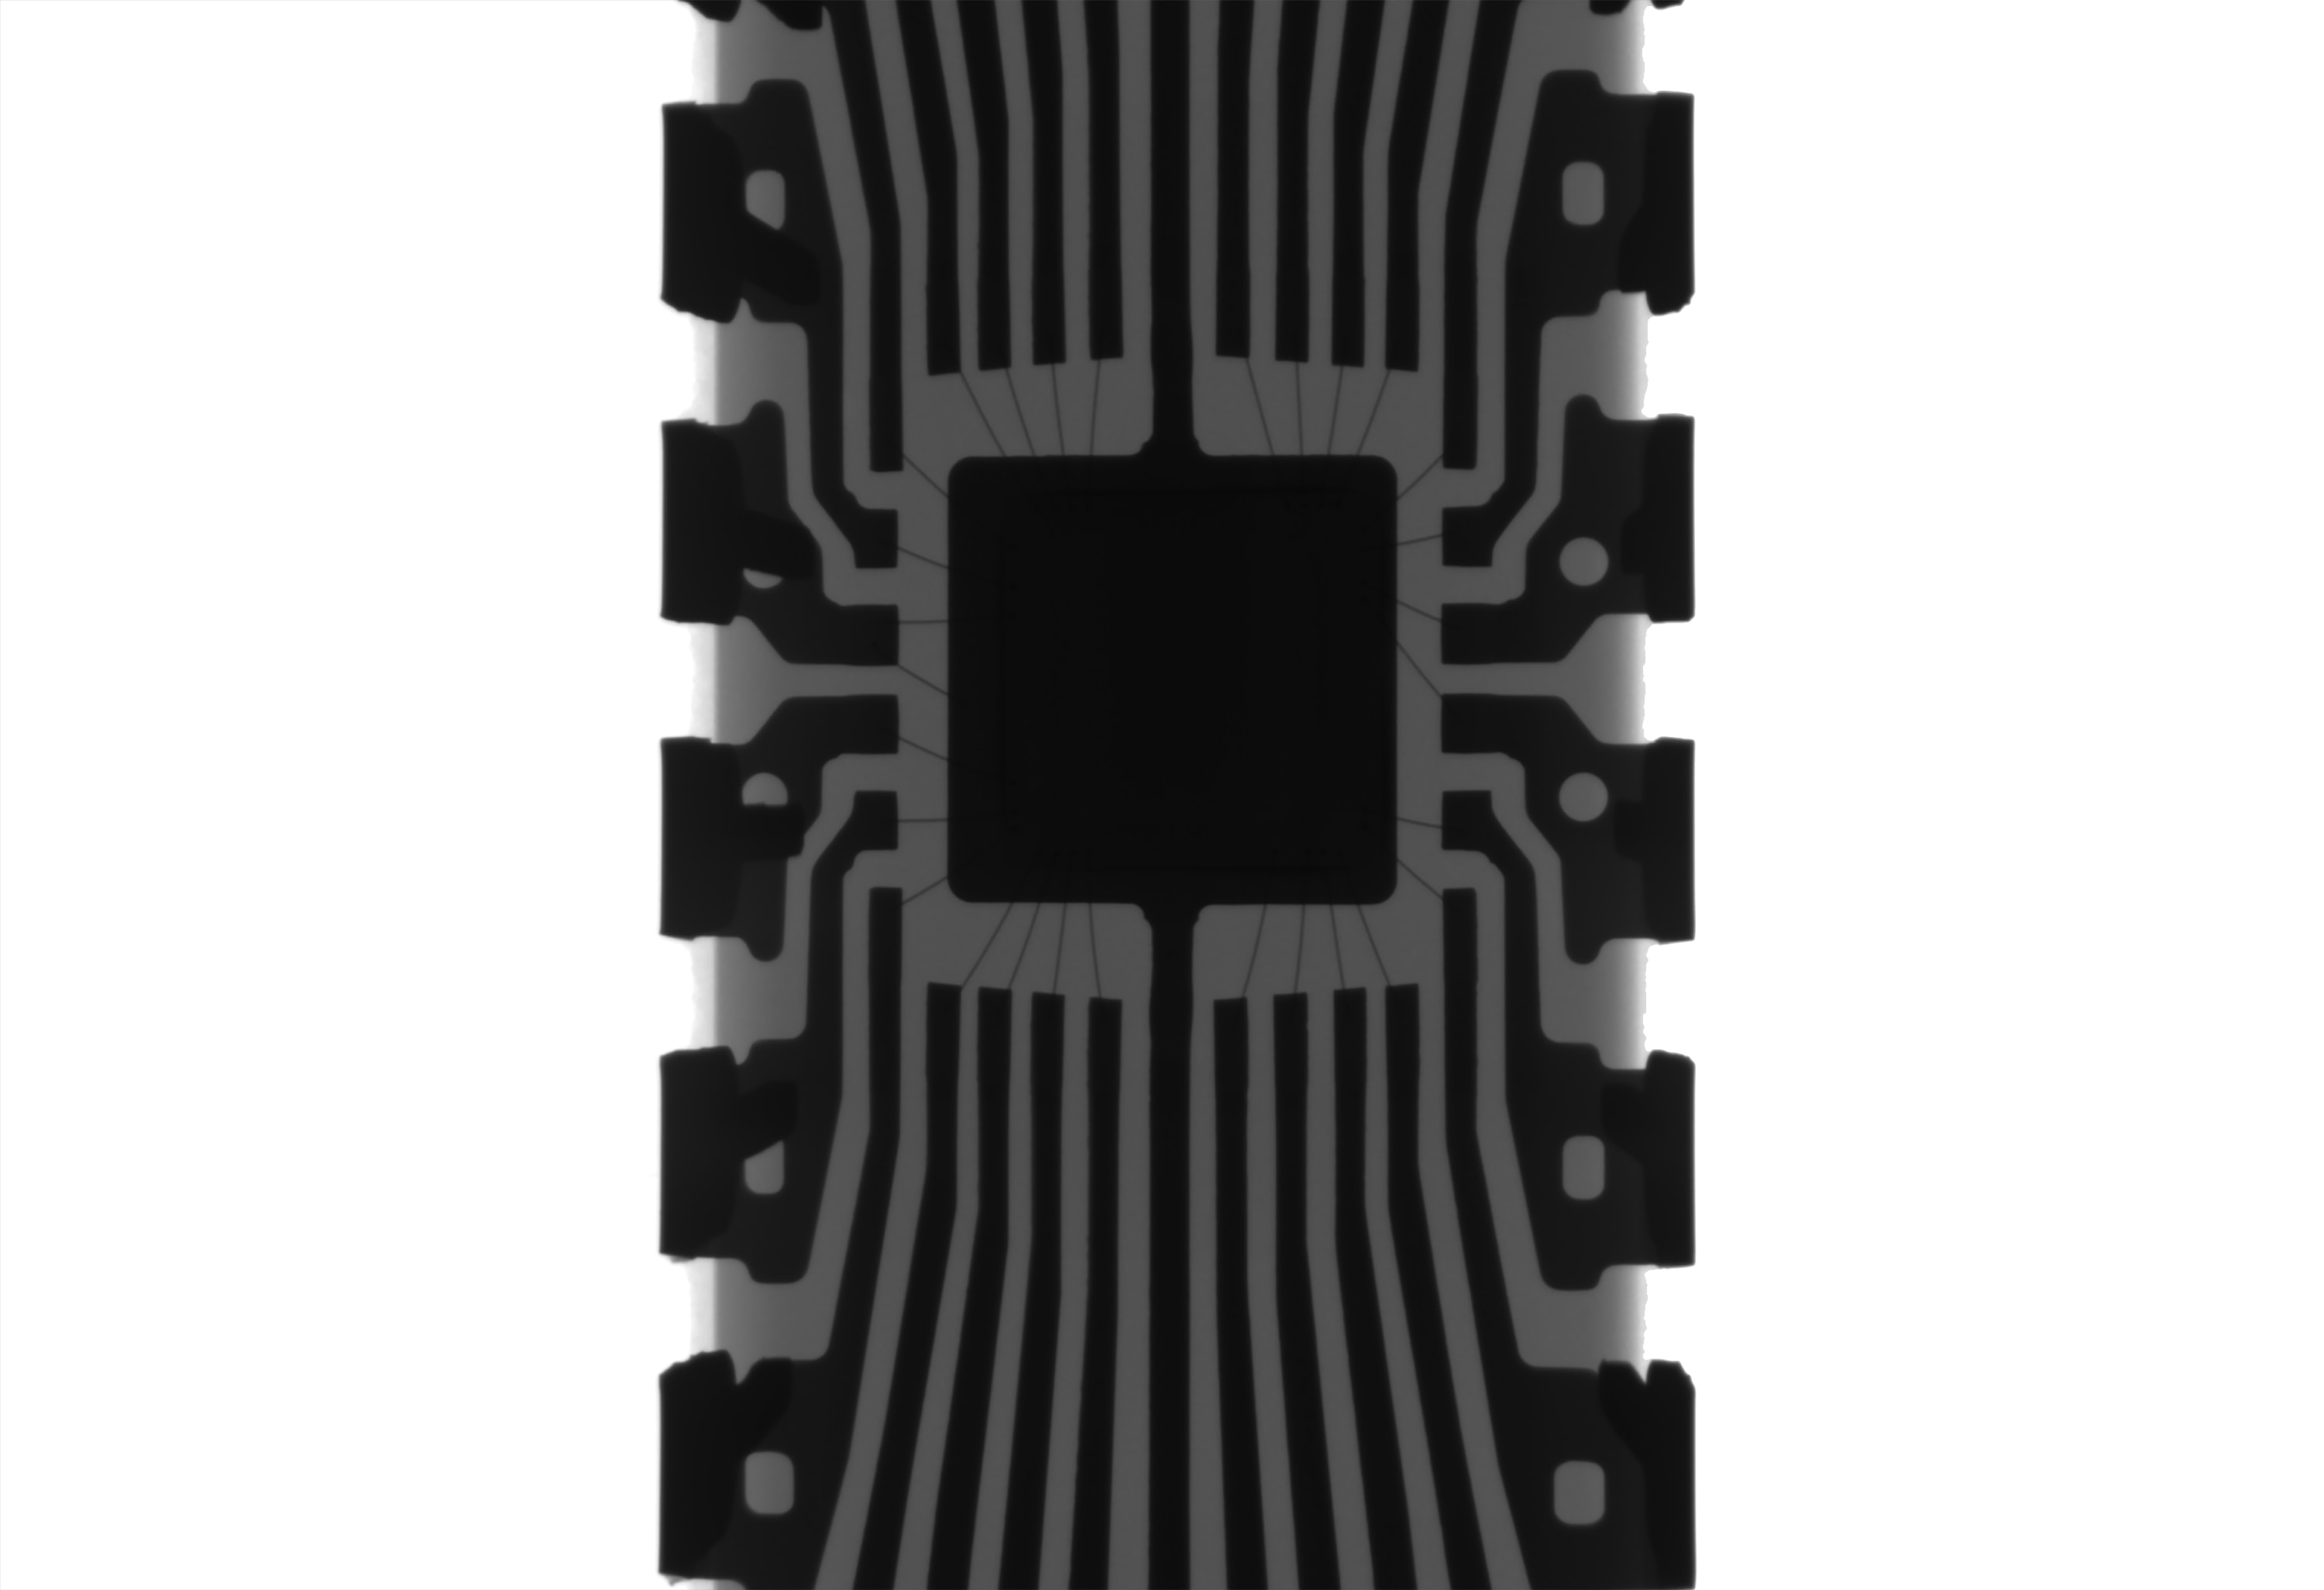
\includegraphics[height=8cm]{img/mathew-schwartz-Il3MNqC5Q1E-unsplash.jpg}
\centering
\end{figure}
\vspace{7cm}

\large
\begin{doublespacing}
\hypersetup{
    urlcolor=black,
  }\urlstyle{same}
  \centerline{GitHub: \url{https://github.com/klaids}}

%\vspace{21em}

\centerline{Last Update on: 27/05/2021}
\end{doublespacing}
\newpage
\tableofcontents
\clearpage
\pagenumbering{arabic}
\newpage
\section{DC CIRCUIT}
\subsection{DC-01}
\begin{figure}[h]
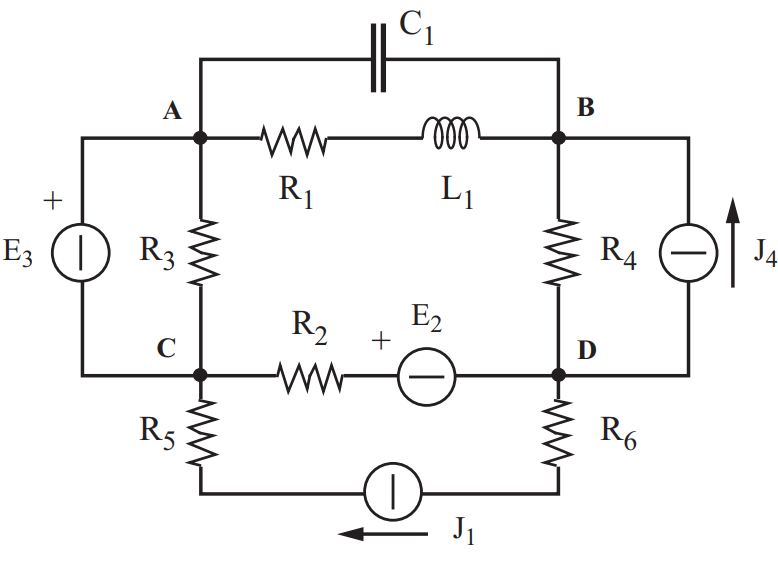
\includegraphics[height=6cm]{img/1/01.png}
\centering
\end{figure}
\begin{center}
\begin{tabular}{ c c c c }
  $R_1 = 2\ \Omega $ & $R_2 = 2\ \Omega$ & $R_3 = 5\ \Omega$ & $R_4 = 1\ \Omega $\\
  $R_5 = 2\ \Omega $ & $R_6 = 1\ \Omega $& $C_1 = 200\ \mu F $& $L_1 = 10\ mH $\\
  $E_3 = 40\ V$ & $J_1 = 20\ A$ & $J_4 = 5\ A$ & $P\ped{R2}=0\ W$\\
\end{tabular}
\end{center}
\underline{\large{Solution:}}
\newline
I\ped{R3}=8\ A, I\ped{E3}=28\ A, I\ped{R4}=25\ A, U\ped{J4}=25\ V
\newline
I\ped{R1}=20\ A, U\ped{C1}=40\ V, E\ped{2}=25\ V, U\ped{J1}=85\ V
\newline
P\ped{R3}=320\ W, P\ped{R4}=625\ W, P\ped{E3}=1120\ W, P\ped{J4}=125\ W
\newline
W\ped{C1}=0.16\ J, W\ped{L1}=2\ J, P\ped{J1}=1700\ W 
\subsection{DC-02}
\begin{figure}[h]
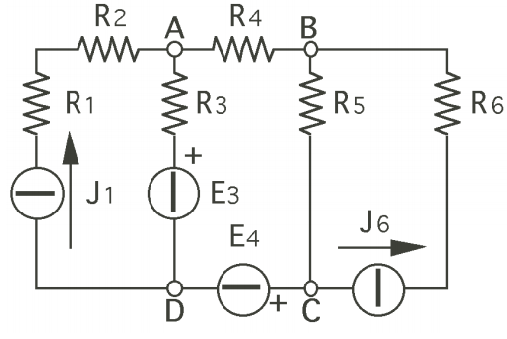
\includegraphics[height=6cm]{img/1/02.png}
\centering
\end{figure}
\begin{center}
\begin{tabular}{ c c c c c}
  $R_1 = 1.5 \ \Omega$ & $R_2 = 2.5 \ \Omega$ & $R_3 = 4 \ \Omega$ & $R_4 = 5 \ \Omega$ & $R_5 = 8 \ \Omega$\\
  $R_6 = 3.5\ \Omega$ & $J_1 = 5\ A$ & $E_3 = 100\ V $& $E_4 = 50\ V$ & $P\ped{J1} = 100\ W$ \\
\end{tabular}
\end{center}
\underline{\large{Solution:}}
\newline
U\ped{J1} = 20\ V, U\ped{AD} = 0\ V, J\ped{6} = -55\ A, U\ped{J6} = -392.5\ V, P\ped{R3} = 2500\ W
\newline
I\ped{E4} = -30\ A, P\ped{R4} = 4500\ W, P\ped{J6} = 21587.5\ W, U\ped{BC} = -200\ V
\subsection{DC-03}
\begin{figure}[h]
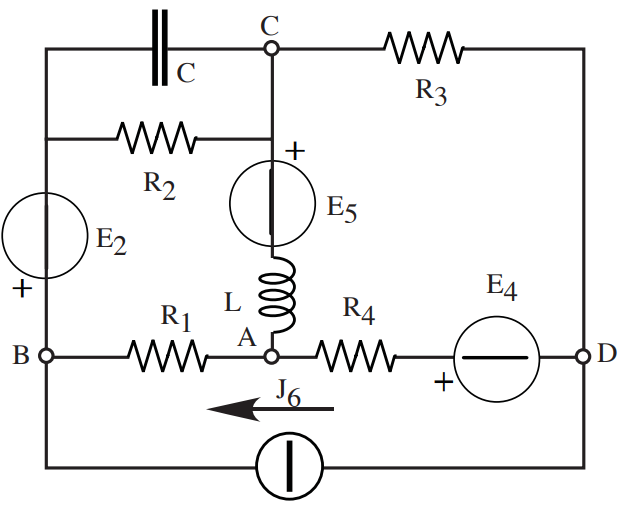
\includegraphics[height=6cm]{img/1/03.png}
\centering
\end{figure}
\begin{center}
\begin{tabular}{ c c c c c}
  $R_1 = 20 \ \Omega$ & $R_2 = 40 \ \Omega$ & $R_3 = 50 \ \Omega$ & $R_4 = 20 \ \Omega$ & $L = 10 \ mH$\\
  $C = 20\ \mu F $ & $E_2 = -900\ V$ & $E_4 = 100\ V $& $E_5 = 800\ V$ & $J_6 = 25\ A$ \\
\end{tabular}
\end{center}
Assuming V\ped{A} = 0, \textbf{determine}:
\begin{itemize}
  \item V\ped{B},V\ped{C},V\ped{D} potentials.
  \item The values of the stored energies W\ped{L} and W\ped{C} respectively from the inductor and capacitor. 
  \item The value of the power P\ped{R\ped{3}} absorbed by resistor R\ped{3}. 
\end{itemize}
\underline{\large{Solution:}}
\vspace{0.2cm}
%ET03-12-03_staz_soluzione
\begin{center}
$J\ped{2}=\frac{E\ped{2}}{R\ped{2}}= -22,5\ A$ \hspace{0.5cm} $G\ped{2}=\frac{1}{R\ped{2}}= 1/40\ S$
\\
\vspace{0.2cm}
$J\ped{4}=\frac{E\ped{4}}{R\ped{4}}= 5\ A$ \hspace{0.5cm} $G\ped{4}=\frac{1}{R\ped{4}}= 1/20\ S$
\[
\begin{cases}
J\ped{6}+J\ped{2} = V\ped{B}\ (G\ped{1}+G\ped{2})-V\ped{C}G\ped{2}\\
I\ped{E\ped{5}}-J\ped{2} = -V\ped{B}G\ped{2}+V\ped{C}\ (G\ped{2}+G\ped{3})-V\ped{D}G\ped{3}\\
-J\ped{4}-J\ped{2} = -V\ped{C}G\ped{3} +V\ped{D}\ (G\ped{3}+G\ped{4})\\
V\ped{C}-V\ped{A}=E\ped{5}
\end{cases}
\]
\[
\begin{cases}
V\ped{B}= \dfrac{J\ped{2} + J\ped{6} + E\ped{5}G\ped{2} }{G\ped{1} + G\ped{2}} = 300\ V\\
V\ped{C} = E\ped{5} = 800\ V\\
V\ped{D}= \dfrac{-J\ped{4} - J\ped{6} + E\ped{5}G\ped{3} }{G\ped{3} + G\ped{4}} = -200\ V\\
I\ped{E\ped{5}} = J\ped{2} - V\ped{B}G\ped{2}+V\ped{C}(G\ped{2} + G\ped{3})-V\ped{D}G\ped{3} =10\ A
\end{cases}
\]
\\
\vspace{0.3cm}
$U\ped{C} = E\ped{2} + (V\ped{C} - V\ped{B}) = -400\ V$\\
\vspace{0.2cm}
$W\ped{C} =\dfrac{1}{2}CU\ped{C}^2= 1,6\ J$\\
\vspace{0.2cm}
$W\ped{L} =\dfrac{1}{2}LI\ped{L}^2=\dfrac{1}{2}LI\ped{E\ped{5}}^2= 0,5\ J$\\
\vspace{0.2cm}
$P\ped{R\ped{3}} =(V\ped{C} - V\ped{D})^2\ G\ped{3}= 20\ \si{\kilo}W$\\
\end{center}
\vspace{1cm}
\subsection{DC-04}
\begin{figure}[h]
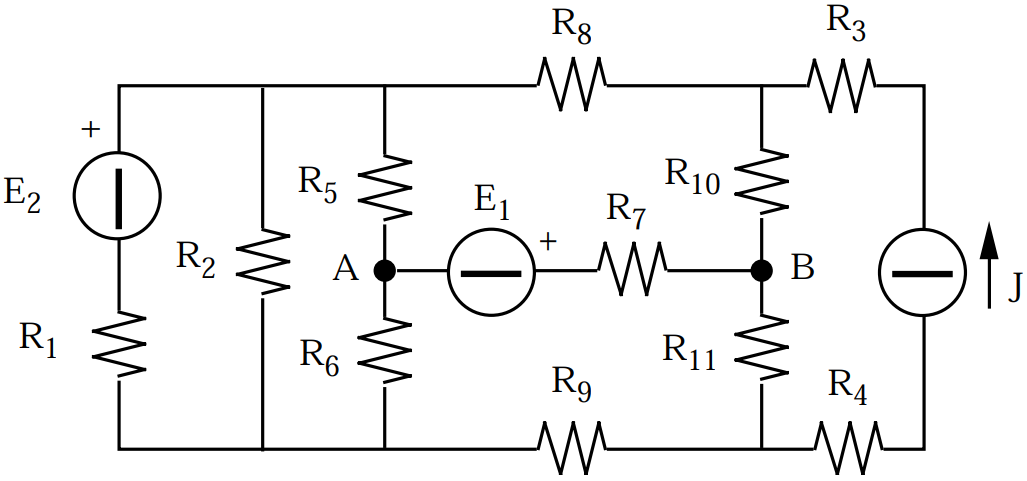
\includegraphics[height=6cm]{img/1/04.png}
\centering
\end{figure}
\begin{center}
\begin{tabular}{ c c c c c}
  $R_1 = 60 \ \Omega$ & $R_2 = 60 \ \Omega$ & $R_3 = 15 \ \Omega$ & $R_7 = 50 \ \Omega$ & $R_4 = 15 \ \Omega$\\
  $R_5 = 15\ \Omega$ & $R_6 = 15\ \Omega$ & $R_8 = 6 \ \Omega$& $R_9 = 4 \ \Omega$ & $R\ped{10} = 10 \ \Omega$ \\
  $R\ped{11} = 10 \ \Omega$ & $E_2 = 180 \ V$ & $J = 9 \ A$ & $P\ped{R7} = 0 \ W$ \\
\end{tabular}
\end{center}
\textbf{Determine}:
\begin{itemize}
  \item E\ped{1}.
  \item P\ped{J1}, P\ped{E2}. 
  \item P\ped{R8}, P\ped{R9}. 
\end{itemize}
\underline{\large{Solution:}}
\newline
E\ped{1} = 3\ V, P\ped{J1} = 3510\ W, P\ped{E2} = 270\ W, P\ped{R8} 54\ W, P\ped{R9} = 36\ W
\subsection{DC-05}
\begin{figure}[h]
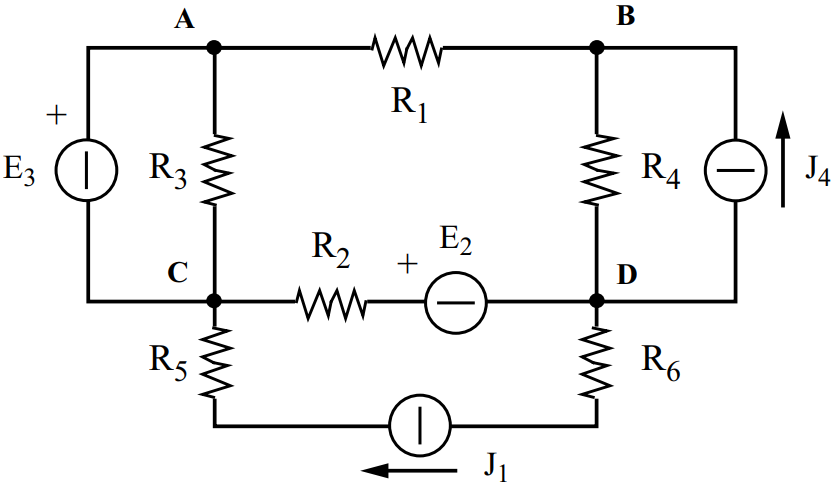
\includegraphics[height=6cm]{img/1/05.png}
\centering
\end{figure}
\begin{center}
\begin{tabular}{ c c c c c}
  $R_1 = 2 \ \Omega$ & $R_2 = 2 \ \Omega$ & $R_3 = 5 \ \Omega$ & $R_4 = 1 \ \Omega$ & $R_5 = 2 \ \Omega$\\
  $R_6 = 1\ \Omega$ & $E_3 = 80\ V$ & $J_1 = 40 \ A$& $J_4 = 10 \ A$& $P\ped{R2} = 0 \ W$  \\
\end{tabular}
\end{center}
\newpage
\textbf{Determine}:
\begin{itemize}
  \item P\ped{R3}, P\ped{R4}
  \item P\ped{E3}, P\ped{J4}.
  \item E\ped{2}. 
  \item P\ped{J1}. 
\end{itemize}
\underline{\large{Solution:}}
\newline
P\ped{R3} = 1280\ W, P\ped{R4} = 2500\ W, P\ped{E3} = 4480\ W, P\ped{J4} = 500\ W, E\ped{2} = 50\ V, P\ped{J1} = 6800\ W
\subsection{DC-06}
\begin{figure}[h]
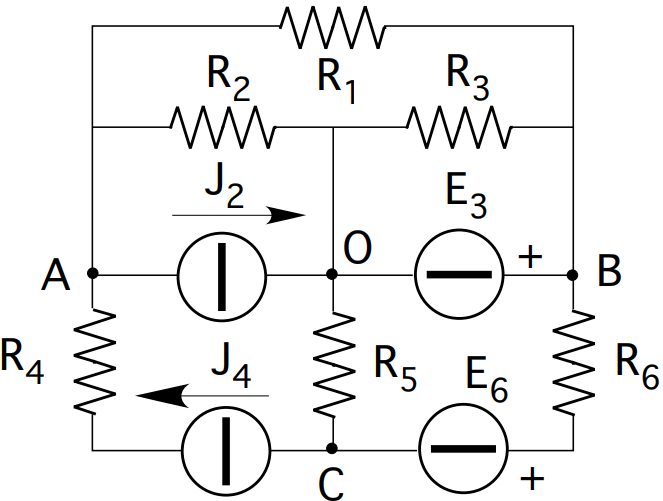
\includegraphics[height=6cm]{img/1/06.png}
\centering
\end{figure}
\begin{center}
\begin{tabular}{ c c c c c}
  $R_1 = 20 \ \Omega$ & $R_2 = 30 \ \Omega$ & $R_3 = 30 \ \Omega$ & $R_4 = 30 \ \Omega$ & $R_5 = 20 \ \Omega$\\
  $R_6 = 12\ \Omega$ & $J_2 = 17.5\ A$ & $J_4 = 4 \ A$& $E_3 = 120 \ V$& $E\ped{6} = -168 \ V$  \\
\end{tabular}
\end{center}
Assuming V\ped{O} = 0\ V, \textbf{determine}:
\begin{itemize}
  \item V\ped{A},V\ped{B},V\ped{C} potentials.
  \item P\ped{J2}, P\ped{E3}, P\ped{J4}, P\ped{E6}. 
\end{itemize}
\underline{\large{Solution:}}
\newline
V\ped{A} = -90\ V, V\ped{B} = 120\ V, V\ped{C} = 150\ V, P\ped{J2} = 1575\ W, P\ped{E3} = 3120\ W, P\ped{J4} = -480\ W\\ P\ped{E6} = 1932\ W.
\newpage
\subsection{DC-07}
\begin{figure}[h]
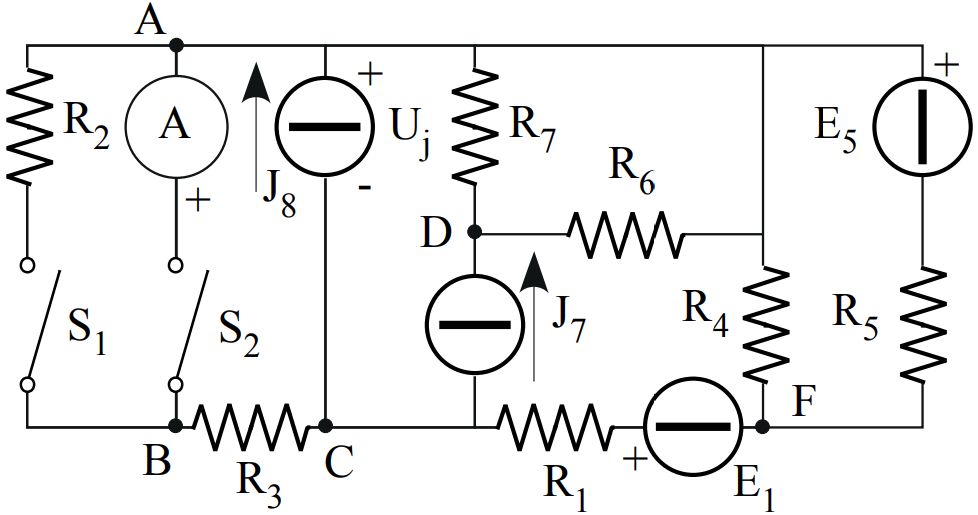
\includegraphics[height=6cm]{img/1/07.png}
\centering
\end{figure}
\begin{center}
\begin{tabular}{ c c c c c}
  $I_A = 20 \ A$ & $P\ped{R2} = 5120\ W$ & $R_2 = 20 \ \Omega$
  $R_3 = R_5 = R_1$ & $R_4 = R_6 = R_7 = 2R_1$
\end{tabular}
\end{center}
I\ped{A} when S1 open and S2 close. P\ped{R2} when S1 close and S2 open, \textbf{determine}:
\begin{itemize}
  \item R\ped{1}.
  \item U\ped{J} when both switches are open.
  \item $P^{'}_{R3}$ and $U^{'}_{j}$ when S1 close and S2 open.
\end{itemize}
\underline{\large{Solution:}}
\newline
$R\ped{1} = 30\ \Omega$, U\ped{J} = -1600\ V, $P^{'}_{R3}$ = 7680\ W, $U^{'}_{j}$ = -800\ V.
\subsection{DC-08}
\begin{figure}[h]
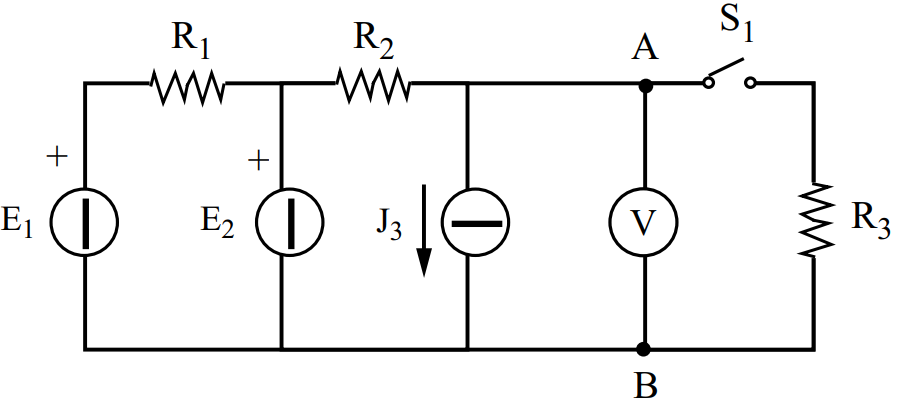
\includegraphics[height=6cm]{img/1/08.png}
\centering
\end{figure}
\begin{center}
\begin{tabular}{ c c c }
  $E_1 = 120 \ V$ & $J_3 = 4\ A$ & $R_1 = 10 \ \Omega$\\
  $R_2 = 10 \ \Omega$ & $R_3 = 20 \ \Omega$ & $U_V = 60\ V$
\end{tabular}
\end{center}
\newpage
U\ped{V} measured when S\ped{1} opened. \textbf{Determine}:
\begin{itemize}
  \item E\ped{2}.
  \item $P\ped{E\ped{1}}$, $P\ped{E\ped{2}}$ and $P\ped{J\ped{3}}$ when S\ped{1} opened.
  \item $U^{'}_{V}$ when $S_1$ closed.
  \item $P^{'}_{E_1}$, $P^{'}_{E_2}$ and $P^{'}_{J_3}$ when $S_1$ closed.
\end{itemize}
\underline{\large{Solution:}}
\newline
$E\ped{2} = 100\ V$, $P\ped{E\ped{1}}$ = 240\ W, $P\ped{E\ped{2}}$ = 200\ W, $P\ped{J\ped{3}}$ = -240\ W, $U^{'}_{V}$ = 40\ V, $P^{'}_{E_1}$ = 240\ W\\ $P^{'}_{E_2}$ = 400\ W, $P^{'}_{J_3}$ = -160\ W.
\subsection{DC-09}
\begin{figure}[h]
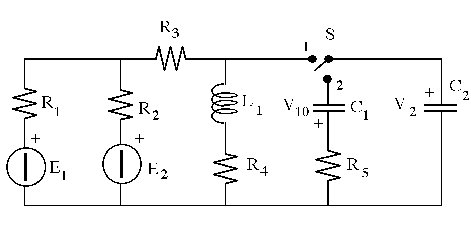
\includegraphics[height=6cm]{img/1/09.pdf}
\centering
\end{figure}
\begin{center}
\begin{tabular}{ c c c c}
  $E_1 = 100 \ V$ & $E_2 = 200\ V$ & $V\ped{10} = 150 \ V$ & $R_1 = 30 \ \Omega$\\
  $R_2 = 20 \ \Omega$ & $R_3 = 13 \ \Omega$ & $R_4 = 75 \ \Omega$ & $R_5 = 75 \ \Omega$\\
  $L_1 = 0.8 \ H$ & $C_1 = 200 \ \mu F$ & $C_2 = 100 \ \mu F$\\
\end{tabular}
\end{center}
 The circuit is in steady state when S is in 1. The capacitor C\ped{1} is charged to voltage V\ped{10}. Then the switch is switched to the position 2. \textbf{Determine}:
\begin{itemize}
  \item The energy W\ped{0} stored overall by the circuit.
  \item The voltage $V^{'}_2$ at the ends of C\ped{1} when S is in position 2.
  \item The electric work $\mathcal{L}\ped{R5}$ absorbed by resistor R\ped{5} when S switched from 1 to 2.
\end{itemize}
\underline{\large{Solution:}}
\newline
$W\ped{0} = 4.25\ J$, $V^{'}_2$ = -60\ V, $\mathcal{L}\ped{R5}$ = 2.43\ J.
\newpage




\section{AC CIRCUIT}
\subsection{AC-01}
\begin{figure}[h]
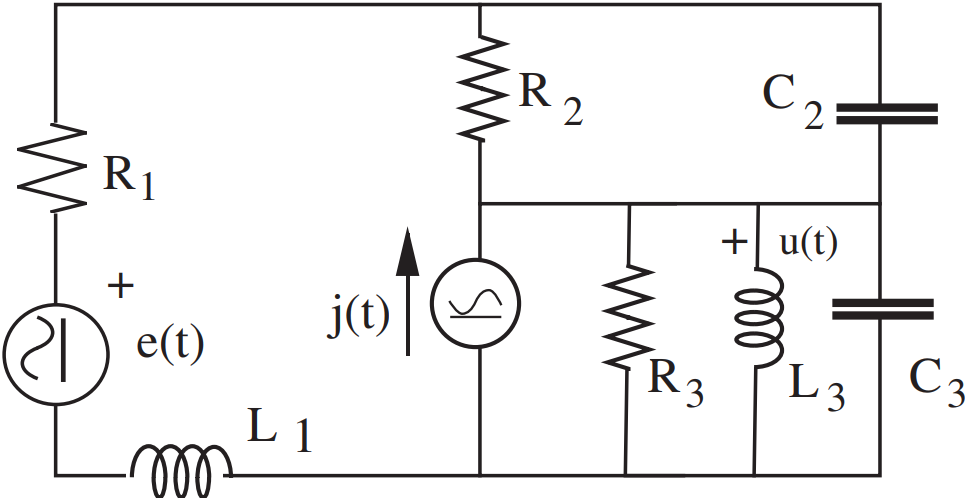
\includegraphics[height=6cm]{img/2/01.png}
\centering
\end{figure}
\begin{center}
\begin{tabular}{ c c c }
  $j(t) = 30\ \sin{(100t + \dfrac{\pi}{4})}$ & $e(t) =300 \sqrt{2} \ \sin{(100t + \dfrac{\pi}{2})}$ & $R_1 = R_3 = 10 \ \Omega$\\
  $R_2 = 20 \ \Omega$ & $L_1 = 400\ mH $ & $L_3 = 400\ mH $\\
  $C_2 = 500 \ \mu F$ & $C_3 = 250 \ \mu F$\\
\end{tabular}
\end{center}
\textbf{Determine}:
\begin{itemize}
  \item $u(t)$
  \item $P\ped{j}$ and $Q\ped{j}$
  \item $P\ped{e}$ and $Q\ped{e}$
\end{itemize}
\underline{\large{Solution:}}
\newline
$u(t) =250 \sqrt{2} \ \sin{(100t + 0.9273)}$, $P\ped{j} = 5250\ W$, $Q\ped{j} = 750\ var$, $P\ped{e} = 1500\ W$\\
$Q\ped{e} = 3.3448\ \cdot 10^{-13}\ var$
\subsection{AC-02}
\begin{figure}[h]
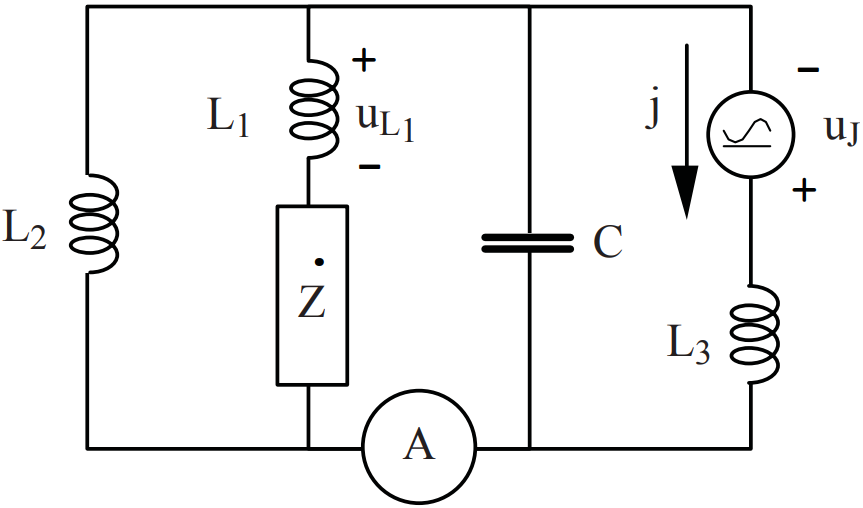
\includegraphics[height=6cm]{img/2/02.png}
\centering
\end{figure}
\begin{center}
\begin{tabular}{ c c c c }
    $L_1 = 10\ mH $ & $L_2 = 15\ mH $ & $L_3 = 15\ mH $ & $C = 25\ \mu F$\\ $u\ped{L_1}(t) = 320\ \cdot\ \sin{(1000t + \dfrac{\pi}{4})}$ & $I_A = 0\ A$
\end{tabular}
\end{center}
\textbf{Determine}:
\begin{itemize}
  \item $\Dot{Z} = R + j X$
  \item $Q\ped{L_2}$
  \item $j(t)$ and  $u\ped{j}(t)$ 
  \item $Q\ped{L_3}$
\end{itemize}
\underline{\large{Solution:}}
\newline
$\Dot{Z} = -25i$, $Q\ped{L_2} = 7680\ var$, $j(t) = 12\ \cdot\ \sin{(1000t + \dfrac{3}{4}\ \pi )}$, $u\ped{j}(t) = 300\ \cdot\ \sin{(1000t + \dfrac{\pi}{4}\ )}$, $Q\ped{L_3} = 1080\ var$
\subsection{AC-03}
\begin{figure}[h]
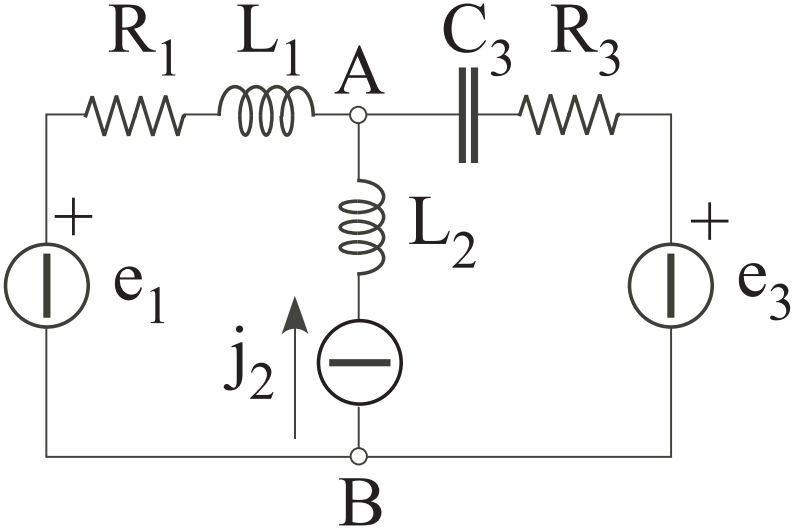
\includegraphics[height=6cm]{img/2/03.png}
\centering
\end{figure}
\begin{center}
\begin{tabular}{ c c c }
    $e\ped{1}(t) = 100\ \sin{(1000t)}$ & $j\ped{2}(t) = 8\ \cos{(1000t)}$ & $e\ped{3}(t) = 200\ \sin{(1000t)}$\\
    $R_1 = 5\ \Omega$ & $R_3 = 10\ \Omega$ & $L_1 = 5\ mH$ \\
    $L_2 = 10\ mH$ & $C_3 = 100\ \mu F$
\end{tabular}
\end{center}
\textbf{Determine}:
\begin{itemize}
  \item $P\ped{R_1}$ and $P\ped{R_3}$
  \item $P\ped{E_1}$, $P\ped{J_2}$ and $P\ped{E_3}$ 
  \item $S\ped{J_2}$ 
  \item $i\ped{e_3}(t)$
\end{itemize}
\underline{\large{Solution:}}
\newline
$P\ped{R_1} = 776\ W$, $P\ped{R_3} = 848\ W$, $P\ped{E_1} = -920\ W$, $P\ped{J_2} = 704\ W$, $P\ped{E_3} = 1840\ W$, $S\ped{J_2} = 729.71\ $VA, $i\ped{e_3}(t) = 13.023\ \sin{(1000t + 0.043451 )}$
\newpage
\subsection{AC-04}
\begin{figure}[h]
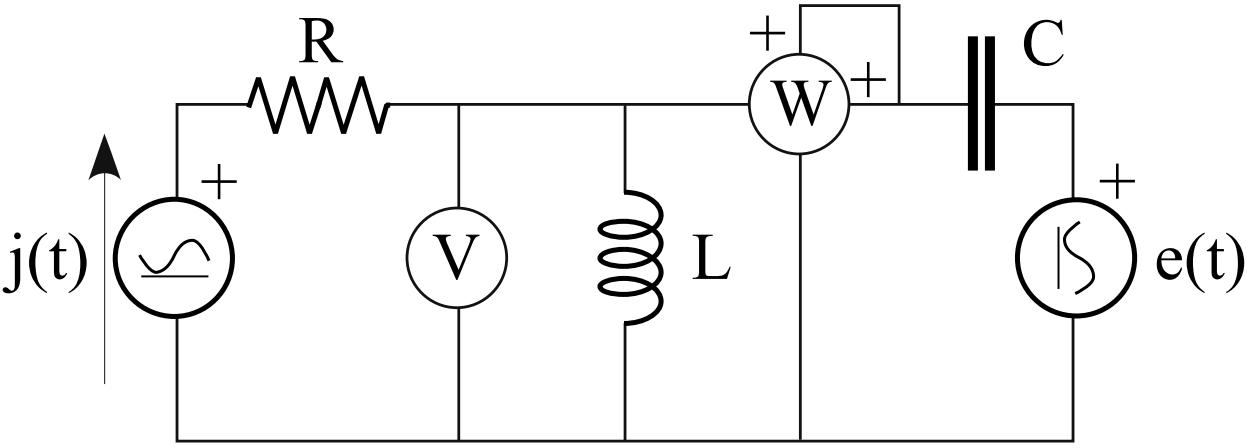
\includegraphics[height=5cm]{img/2/04.png}
\centering
\end{figure}
\begin{center}
\begin{tabular}{ c c c }
    $e(t) = 100 \cdot \sqrt{2}\ \sin{(200t)}$ & $j(t) = 10 \cdot \sqrt{2} \sin{(200t + \pi)}$ & $R = 5\ \Omega$\\
    $L = 100\ mH$ & $C = 500\ \mu F$\\
\end{tabular}
\end{center}
\textbf{Determine}:
\begin{itemize}
  \item The indication of the voltmeter $U_V$
  \item $P\ped{W}$ 
  \item $u\ped{j}(t)$
  \item $i\ped{e}(t)$
  \item $P\ped{j}$ and $Q\ped{j}$
\end{itemize}
\underline{\large{Solution:}}
\newline
$U_V = 282.84\ V$, $P\ped{W} = 2000\ W$, $u\ped{j}(t) = 353.55\ \cdot\ \sin{(200t + 0.9273 )}$, $i\ped{e}(t) = 31.623\ \cdot\ \sin{(200t - 0.46365 )}$\\
$P\ped{j} = -1500\ W$,  $Q\ped{j} = -2000\ var$
\newline

\end{document}
